\chapter{Introduction}
\label{ch:Introduction}
\graphicspath{{Chapter1/Chapter1Figures/}}
As modern technology and machine learning techniques advances, it is important for the educational sector to continuously advance in their learning environment. This allows for an ever improving learning experience in and outside the classroom. 

\section{Problem background}

In the recent years the Applied Mathematics Department of Stellenbosch Engineering, started observing a decrease in accuracy in the grading of tutorial tests done by teaching assistants and demies.  Students complained on a regular basis about correct answers being marked incorrectly or even that their answers were totally ignored. Furthermore, the assistants took a long time to grade these tests with time and financial implications. To address this problem, the Applied Mathematics department proposed to automate the process of grading the tutorial tests.

The head of the department wanted a system that can analyse and grade tests written on a specific template. These answer sheets are handed out to the students to fill in their respective answers. The answer sheets are then scanned to create a digital copy. The system is tasked with automatically grading all these digital copies and transferring the graded results to a database.

The department has tried to use a basic version of this type of system in the past. Such a system only really becomes useful to the department if it can grade decimal valued answers instead of only being able to grade multiple choice answers. Thus a template needs to be designed that allows students to answer with decimal valued answers. Another factor to consider is filling in those values must still be relatively easy. Therefore students need to have the freedom of quickly crossing out an answer instead of erasing it each time.
In this research project the department sends weekly scanned answer sheets, which need to be graded and the results returned to them. The feedback from these weekly tutorial tests then acts as validation tests for the system. These tests are done in parallel with the development and expansion of the test grading software. For these reasons an agile development methodology is used to develop the software.

\section{Problem statement}
\label{sec:problemStatement}

Given the problem background and stakeholders discussed in the previous section the problem to be solved can be formulated as follows:
\newline
\newline
\noindent\fbox{%
    \parbox{\textwidth}{%
    \textbf{Develop} and \textbf{implement} an \textsl{automatic test grading system} that will \textsl{increase marking accuracy} and \textsl{decrease marking time}  on the \textsl{grading} of Applied Mathematics tutorial tests written by students.}%
}

\section{Project scope and assumptions}\label{sec:Scope}
Initial discussions with the department revealed that a specific template can be used. This template allows the image processing software to more accurately determine what the student's intended answer is. The template consists of bubbles that can be filled in as well as blocks for handwritten digits, as shown in Figure \ref{fig:NumbersTemplate}. The focus of this project lies on processing the scanned answer sheet written on the specific template. To use the template the student must fill in his/her student number and question answers in the designated character blocks. They are also required to fill in the bubble underneath each digit, corresponding to that specific digit. Additionally, a bubble next to each question is provided if a negative sign is required.

\begin{figure}[h]
  \centering
  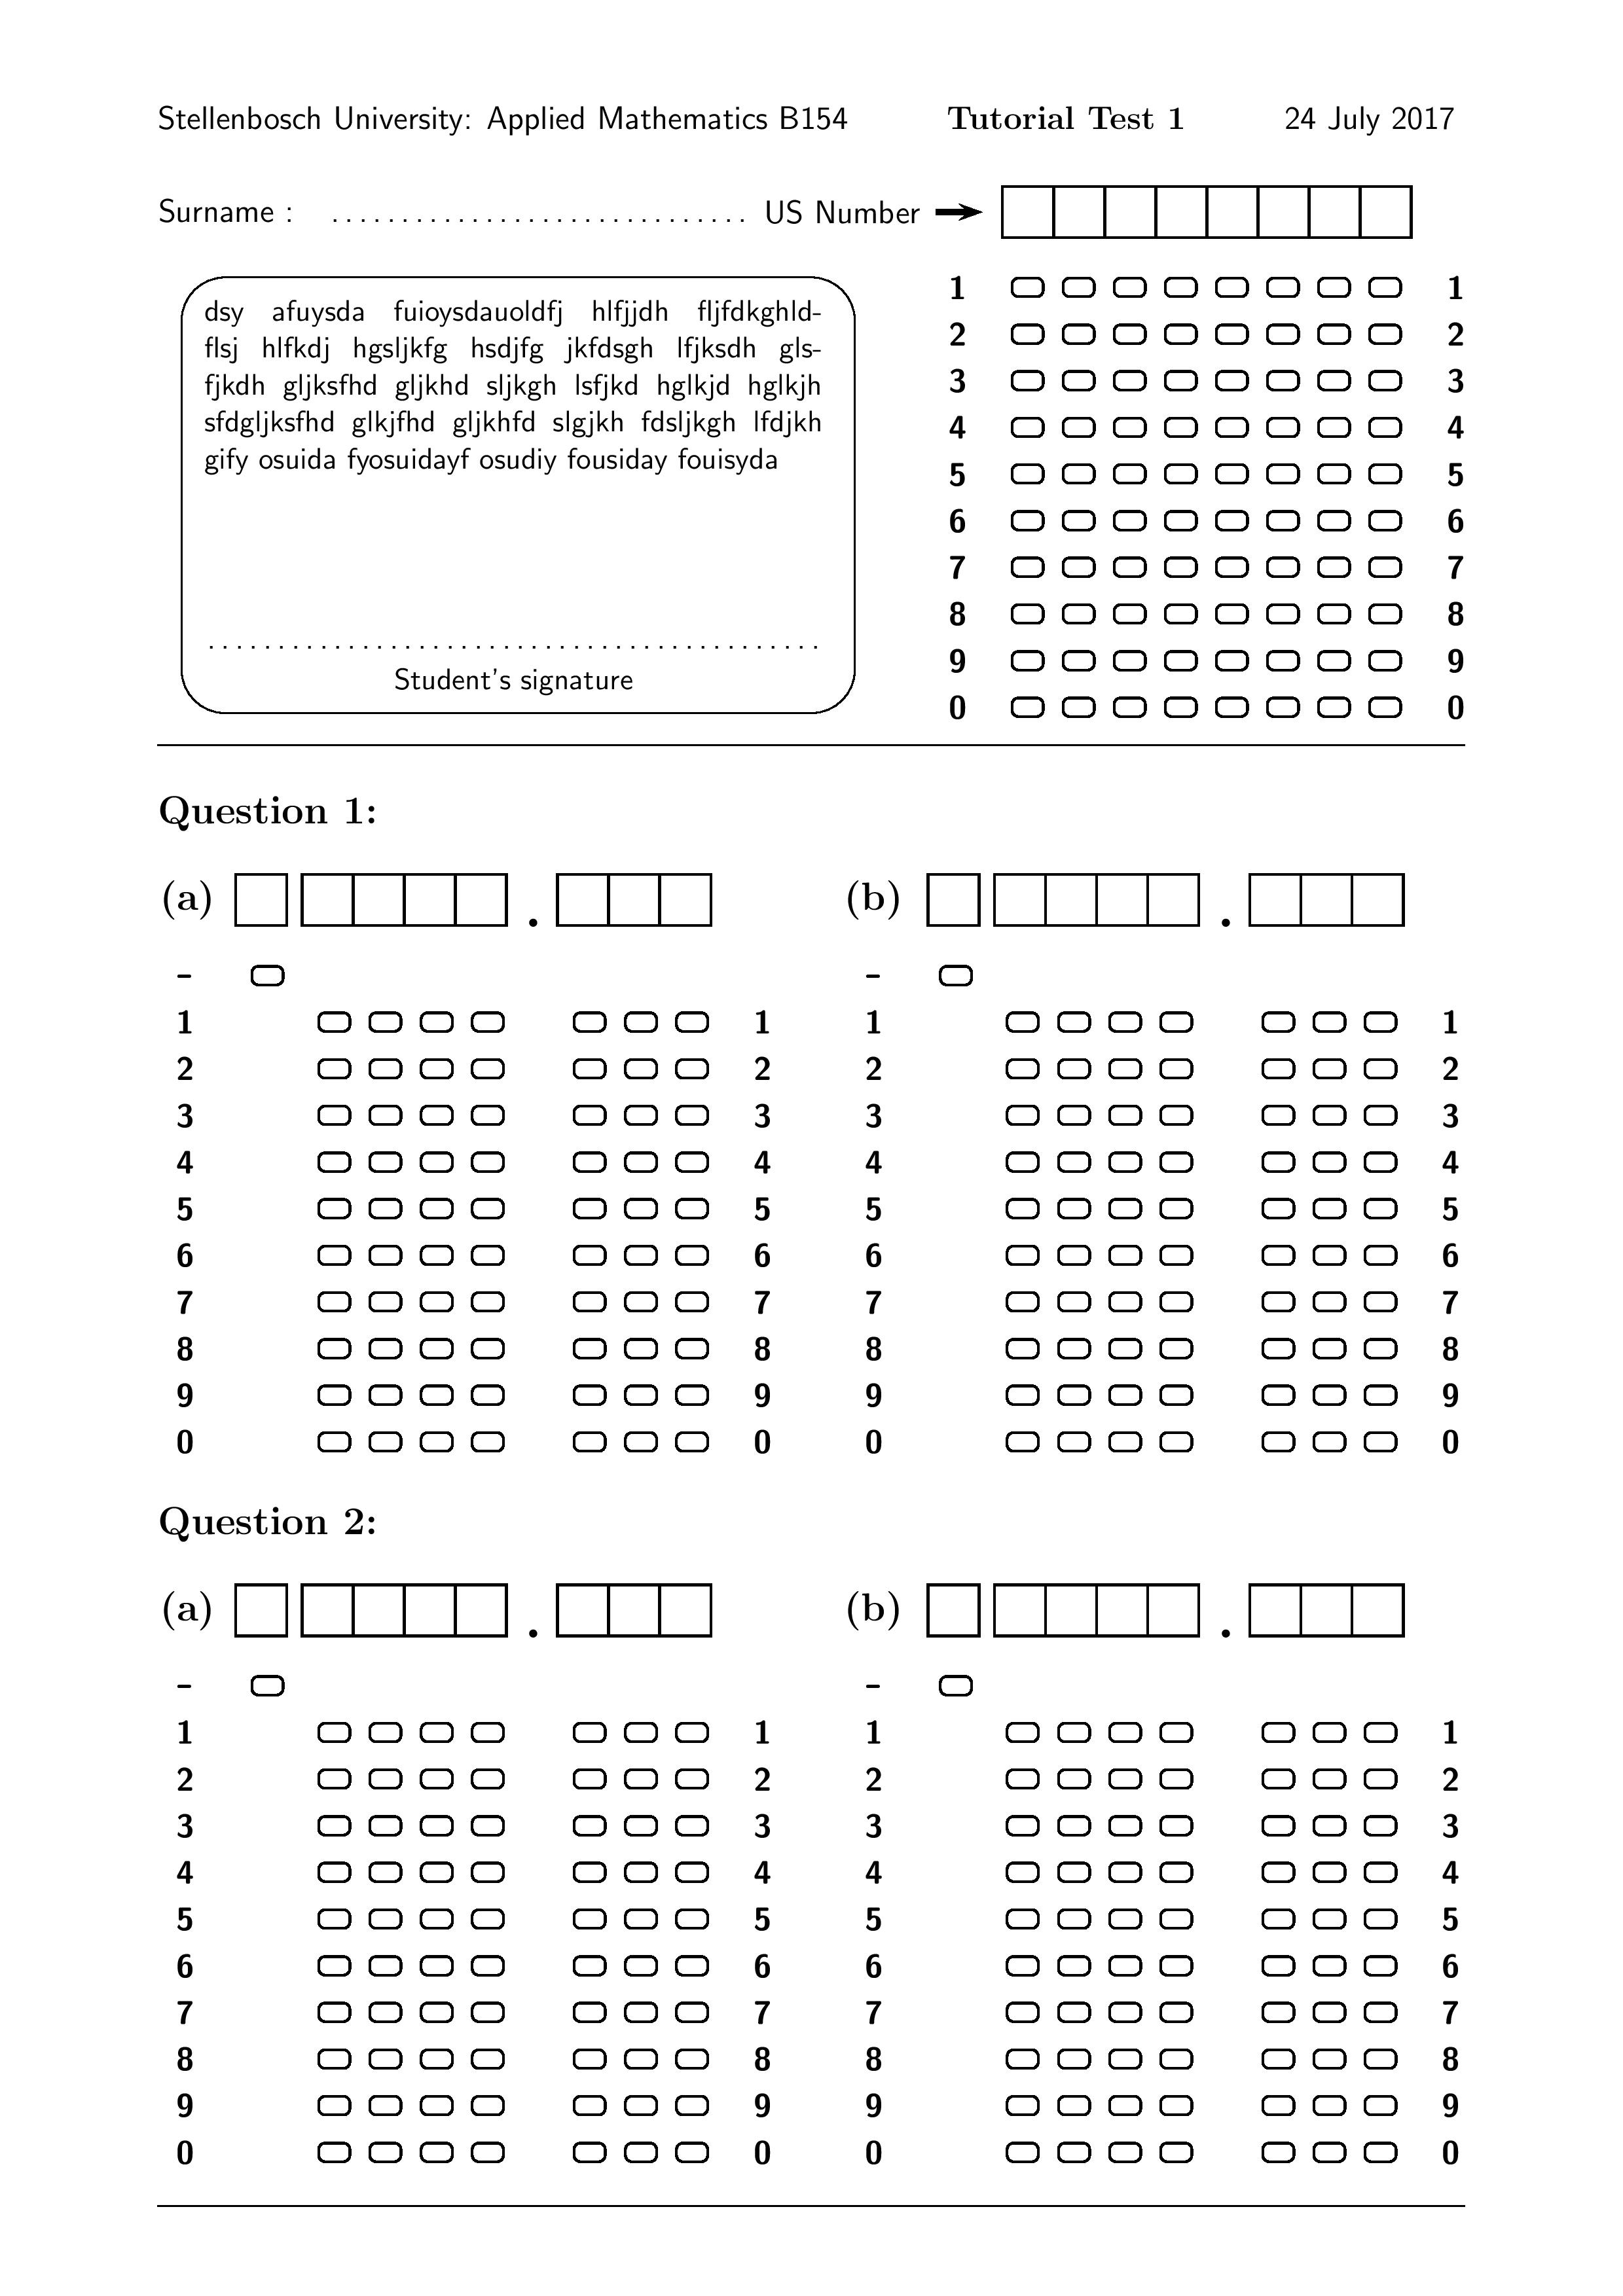
\includegraphics[width=8cm]{NumbersTemplate}\\
  \caption{Automatic test grading template layout.}
  \label{fig:NumbersTemplate}
\end{figure}


Any additional assumptions are stated in the appropriate section throughout this project.


\section{Project objectives}
\label{sec:Objectives}

The problem as stated in Section \ref{sec:problemStatement}, is addressed by pursuing the following objectives:
\begin{enumerate}
  \item Perform a \textsl{literature study} on the topics of \textsl{Image Processing}, \textsl{Computer Vision} and \textsl{Character Recognition}. Further a \textsl{literature study} on \textsl{Neural Networks} and \textsl{Probabilistic Graphical models} is also done.
  \item Develop a \textsl{software application} to allow a \textsl{user} to grade a large number (approximately 1000) scanned student tests automatically.
\item The software should provide precise and useful feedback. In order to achieve this, every graded result will also include feedback on what questions the student answered incorrectly.
\item Upgrade the software to allow students to cross out answers instead of having to erase them.
  \item Do a weekly \textsl{validation experiment} with the software, by grading tutorial test for the department. The results are then used as the students' grades for that test.
  \item Use an \textsl{agile development methodology} to improve the software in parallel with the grading of weekly tests.
  \item Add additional software, using machine learning, to improve the accuracy of the system in grading these tests.
  \item Add additional software that allows students to specify their student number only using characters, thereby simplifying the use of the template.
\end{enumerate}
The objectives are covered in separated chapters in this report. Note that each objective (1 to 8) build on the objectives previously listed.

 %To increase ease of use, software is developed that provides the option to students to only writing down their student numbers and not use the bubbles. Thus time does not get wasted filling in the student number bubbles. This result is achieved in Chapter \ref{sec:pgmStudentNum}.

\section{Research methodology}

An agile development methodology is used to complete the objectives listed in Section \ref{sec:Objectives}. The methodology consists of six different phases:
\begin{enumerate}
\item Identify a new feature or update that needs to be implemented into the software package.
\item Do a study on existing methods to implement this new software.
\item Implement and integrate the new software with the current knowledge of the solution.
\item Test the software and observe if it is working as planned.
\item If the software is not working as planned, revisit steps 2 to 4 until the new software is working.
\item Use version control, in this case Git, to save the latest version of the software.
\end{enumerate}


The structure and graphical overview of the software is presented next.

\section{Graphical overview of system}
The process of writing an answer down on a paper can be represented using 6 information nodes. These nodes are illustrated in Figure \ref{fig:systemOverviewIntro}. The unnamed blocks indicate that information processing occurs in these steps. The student has certain information he/she wants to portray on the paper, namely the 4 answers and student number he/she wants to write down. Thus those 5 nodes give rise to the image, representing the last node. These nodes have to be represented in a probabilistic manner as the process of writing answers down and scanning the test sheet, may produce a different image every time a test is written, even though the same answers are intended. Thus the system is fundamentally tasked with inferring the probability of each answer and the student's number given the particular image as evidence. This is done by processing the image evidence to produce and estimate the intended answers. These processes are described in later sections. In the next section a literature study on current systems is given. For a more detailed mathematical overview of the system, refer to Appendix \ref{ap:systemOverview}.
\\
\\
\\
\\
\begin{figure}[H]
  \centering
  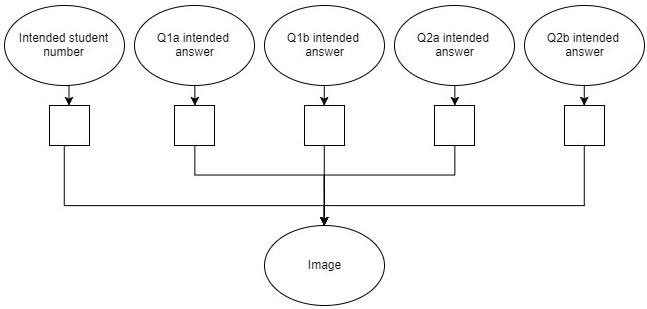
\includegraphics[width=13cm]{systemOverview}\\
  \caption{Graphical overview of the system as a whole.}
  \label{fig:systemOverviewIntro}
\end{figure}